\section{Experiment}
To confirm that NaaA works widely with machine learning tasks,
we confirm our method of supervised learning tasks as well as reinforcement learning tasks.
As supervised learning tasks, we use typical machine learning tasks such as image classification
using MNIST, CIFAR-10, and SVHN.

As reinforcement tasks, we confirm single- and multi-agent environment.
The single-agent environment is from OpenAI gym.
We confirm the result using a simple reinforcement task: CartPole.
In multi-agent, we use ViZDoom, a 3D environment for reinforcement learning.

\subsection{Classification}

\subsubsection{Setup}
In this experiment, we used three types of datasets, MNIST, CIFAR-10 and STL-10. The task given here is to predict the label for each image. The number of class is 10 in those three datasets.
The first dataset, MNIST, is a collection of black and white images of handwritten digits whose size is 28x28. The training set and test setare composed of 60,000 examples and 10,000 examples respectively. 
The images in CIFAR-10 dataset are colored and the size of each image is 32x32. The task is to predict what is shown in each picture. This dataset contains 6,000 images per class (5,000 for training and 1,000 for test).
STL-10 is a dataset for image recognition, the number of which is 1,300 for each class (500 for training and 800 for test). The size of each image is 96x96. In this experiment, however, images were resized into 48x48, since the resolution is large compared to the datasets shown above and this dataset requires far more time and resource to compute.

\subsubsection{Model}
In this experiment, we compared two models, DropConnect and Adaptive DropConnect (proposed model in this paper). The baseline model is composed of two convolutional layers and two fully connected layers whose outputs are dropped out (we set the possibility as 0.5). The labels of input data are predicted using log-softmaxed value of last fully connected layer. In DropConnect model and Adaptive DropConnect model, first fully connected layer is replaced by DropConnected layer  and Adaptive DropConnected layer respectively. Note that DropConnect model corresponds to the our method with $\varepsilon$ = 1.0 and this means agents do not perform their auctions, and randomly mask the weights.

\subsubsection{Results}
For the MNIST datasets, the models are trained for 10 epochs and then evaluated with the test data. The numbers of epochs for CIFAR-10 and STL-10 are 20 and 40 respectively. Experiments are repeated 20 times for each condition, and the average and standard deviation of  error rate was calculated. The results is shown in Table \ref{tbl:cls}. As expected, with the model using Adaptive DropConnect, the classification error rate was lower than both the baseline and DropConnect regardless of the datasets given in this experiment.


\begin{table}[h]
	\caption{ Experimental result for image classification tasks and single-agent RL }\label{tbl:cls}. 
\centering
\begin{tabular}{l|ccc|c}
\hline
		& MNIST & CIFAR-10 & STL-10 & CartPole \\
\hline
		DropConnect \citep{wan2013regularization}	&	1.72 $\pm$ 0.160	&	43.14 $\pm$ 1.335	&	50.92 $\pm$ 1.322 & 285 \\
		Adaptive DropConnect	&	\textbf{1.36} $\pm$ 0.132	&	\textbf{39.84} $\pm$ 1.035	&	\textbf{42.17} $\pm$ 2.329 & \textbf{347} \\
\hline
\end{tabular}
\end{table}

\subsection{Single-agent RL}
Next, we set the single-agent reinforcement learning task.
We used the CartPole task from OpenAI gym with visual input.
In this setting, the agent must balance a pole while moving a cart.
There is much non-useful information related to the image. For that reason, pruning the pixels is important.
The result in Table \ref{tbl:cls} demonstrates that our method improves the standard RL.

\subsection{Multi-agent RL}
The additional feature of NaaA is credit assignment for reward distribution, 
meaning that if the neural network is divided into multiple agents, it works by playing the auction game.
We confirmed that additional agents complement the main player using ViZDoom, an environment for Doom.
A player in Doom environment should seek the enemy in the map, and then defeat the enemy.
Because ViZDoom provides several maps, we used ViZDoom.

\subsubsection{Setup}
We used a scenario based on Defend the Center (DtC), provided by ViZDoom platform.
In DtC, players are placed in the center of a field of circle. They attack enemies that come from the wall.
The game has two players: a main player and a cameraman.
Alhough the main player can attack the enemy with bullets, 
the cameraman has no way to attack, and only scouts for the enemy.
The action space for the main player is the combination of \{ attack, turn left, turn right \}. Therefore, the total number of actions is $2^3 = 8$.
The cameraman has two possible actions: \{ turn left, turn right \}.
Although the players can only change direction, they cannot move on the field.
The enemy will die if have the attack (bullet) from the main player once, then player receives +1.
As a default on an episode, the ammunition amount is 26.
The main player will die if under attack from the enemy to the extent that health becomes 0, then the player receives -1.
The cameraman will not die if attacked by the enemy.
The episode will terminate when the maim player dies, or after 525 steps have elapsed.

\subsubsection{Model}
We compared three models: the proposed method and two comparison targets.

{\em Baseline} DQN without communication. The main player learns standard DQN with the perspective that the player is viewing.
Because the cameraman does not learn, the player continues to move randomly.

{\em Comm} DQN with communication. The main player learns DQN with two perspectives: the player's own and the cameraman's.
The communication vector is learned with a feed-forward neural network. The method is inspired by Commnet.

{\em NaaA} The proposed method. The main player learns DQN with two perspectives: the player's own and the cameraman's.
The transmission of reward and communication are performed using the proposed method.

\begin{figure*}[t]
\centering
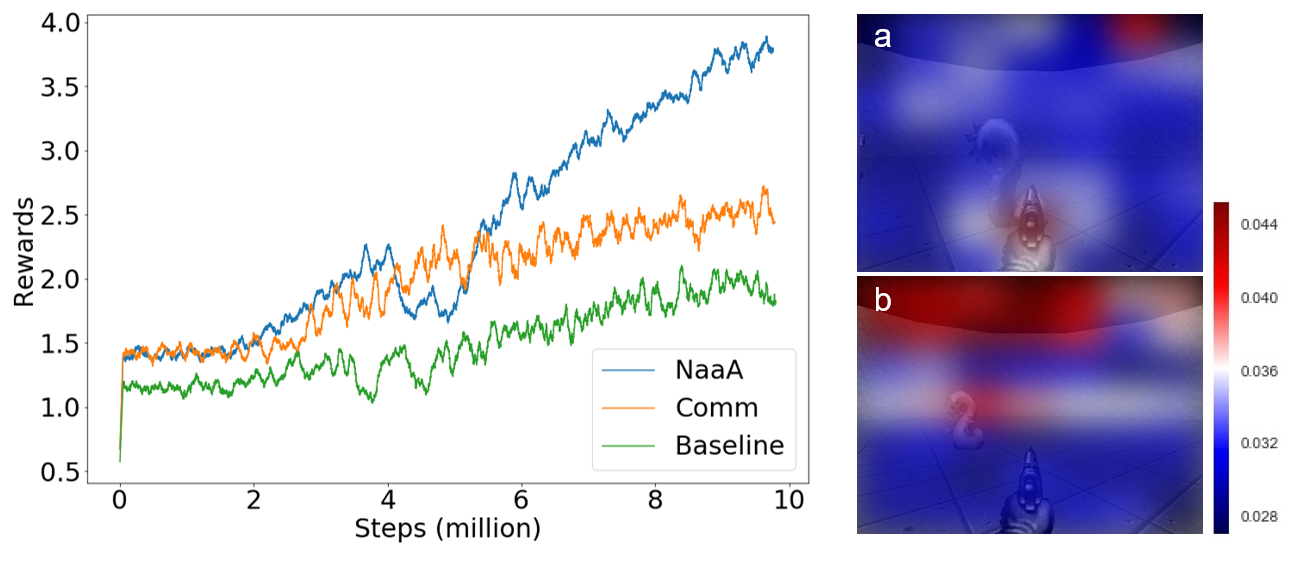
\includegraphics[width=\linewidth]{img/lc_vis.eps}
\caption{
	\textbf{Left:}
		Learning curve for the multi-agent task of VizDoom. 
		Our method based on NaaA outperforms the other two methods: baseline and Comm DQN.
	\textbf{Right:} 
		Reward visualization shows us what the cameraman sees:
		(a) The cameraman sees the pistol.
		(b) The cameraman sees the point which enemy appear and come closer.
}
\label{fig:lc_vis}
\end{figure*}

\begin{figure*}[t]
\centering
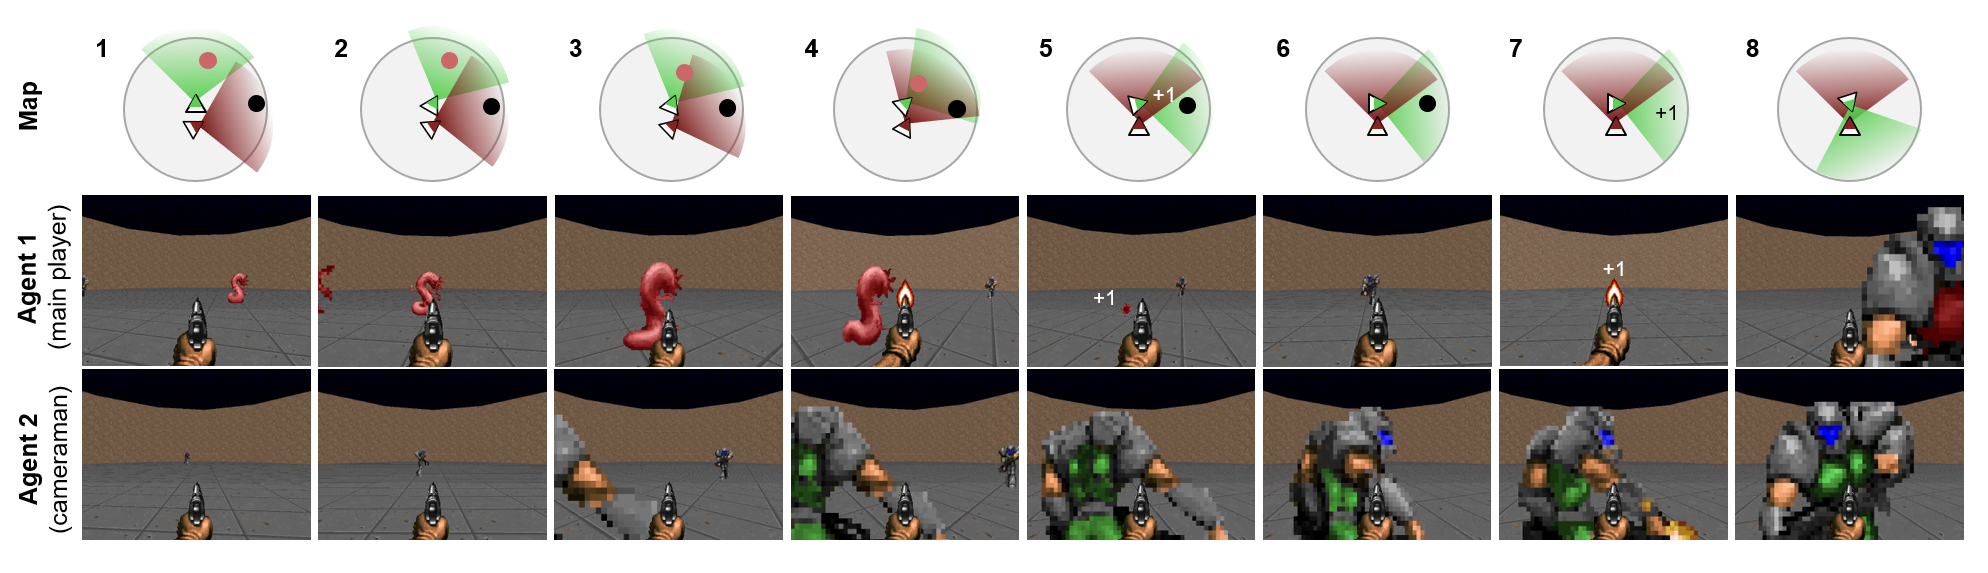
\includegraphics[width=\linewidth]{img/circleworld.eps}
\caption{
NaaA leads the agents to obtain cooperative relationship.
First, the two agents are facing in different directions,
and the cameraman sells its information to the main player (\textbf{1}).
The main player who bought the information starts to turn right to find the enemy.
The cameraman who sold the information starts to turn left to seek new information by finding the blind area of the main player (\textbf{2} and \textbf{3}).
With turning, the main player attacks the first enemy which he already saw (\textbf{4} and \textbf{5}).
After the main player finds out the enemy, he attacks the enemy, and obtain the reward  (\textbf{6} and \textbf{7}).
Until the next enemy appears, the agents watch their dead area each other (\textbf{8}).
}
\label{fig:circleworld}
\end{figure*}

\subsubsection{Results}
Training is performed in 10 million steps.
Figure \ref{fig:lc_vis} Left presents that our model NaaA outperforms two methods.
Improvement is achieved by Adaptive DropConnect.
We confirmed that the cameraman sees the enemy through an episode.
This can be interpreted as the cameraman reporting the enemy position.
In addition to seeing the enemy, the cameraman sees the area behind of main player several times.
This action enables the cameraman to observe attacks from the enemy while seizing a better relative position.

For further interpretation of the result, 
we present visualization of the revenue that the agent earned in Figure \ref{fig:lc_vis} Right as a heatmap.
The background picture is a screen in Doom taken at the moment when the filter in CNN is mostly activated.
%The center corresponds to a position with the enemy appearing far away.
%The top corresponds to a position with the enemy coming closer.
%(b) shows that the agent sees the pistol.
Figure \ref{fig:circleworld} shows an example of learnt sequence of actions by our method.

